\documentclass{beamer}
\usetheme{Berlin}
\usecolortheme{beaver}
\usepackage{graphicx}
\usepackage[export]{adjustbox}
\usepackage{tikz}
\usetikzlibrary{arrows}
\usepackage{amsmath}
\usepackage{lmodern}% http://ctan.org/pkg/lm
\usepackage{mathtools}

\title{Chapter 9}
\subtitle{}
\author[Riccardo \and Eren]{Riccardo~Miccini\inst{1} \and Eren~Can~\inst{1}}
\institute[DTU]
{
	\inst{1}
	Technical University of Denmark\\
	Digital Communication
}
\date{\today}
\subject{Digital Communication}

\tikzstyle{int}=[draw, fill=blue!20]
\tikzstyle{every node}=[font=\tiny]

\begin{document}


	\frame{\titlepage}
	\begin{frame}
		\frametitle{The Matched Filter}
		\begin{itemize}
			\item For a given choice of $s_1(t)$ and $s_2(t)$, we wish to determine an $H(f)$ that maximizes;
			\item The problem is to find to maximise $\mu$=$g_o(T)$
			\item $\zeta=(s_{02}(T)-s_{01}(T))/\sigma_0$
			\item We can equally consider the maximization of ; $\zeta^2=g^2_0(T)/\sigma^2_0$
			\item Since the input noise is stationary, $E(n^2_0(t)) = N_0^2(T) =N_0/2 * \int_{-\infty}^{+\infty} |H(f)|^2 df $
			\item For maximising this equation with respect to $H(f)$, we use the Schwarz's inequality is a generalization of the inequality.
			\item $|A*B|=|A*B*cos(\theta)| < |A|*|B| $, where A and B are
			\item After the following the assumptions , we will get the $h_0(t)$=$g(T-t)$-$s_1(T-t)$
		\end{itemize}
	\end{frame}

	\begin{frame}
		\frametitle{Error Probability for the Matched-Filter Receiver}
		\begin{itemize}
			\item $ P_E = Q(\mu/2) $, where $ \mu $ has the maximum value.
			\item We can use the Parseval's theorem , we can write $\mu^2$ in terms of $g(t)=s_2(t)-s_1(t)$ as
			\item $\mu^2=(2/N_o)*(\int_{-\infty}^{+\infty } (s_2(t)*s_1(t))^2 dt $
			\item We have assumed that $s_1$ and $s_2$ were assumed real and we know that $s_1$ and $s_2$ are the energies for $E_1$ and $E_2$ so than we  define; $\rho_{12}= 1/(\sqrt{E_1, E_2}) * \int_{-\infty}^{+\infty} (s_2(t)*s_1(t))^2 dt$
			\item We know that $s_1(t)$ and $s_2(t)$ are correlation coefficients of $s_1(t)$ and $s_2(t)$ and it is normalized such that $-1 < \rho_12 < 1$
		\end{itemize}
	\end{frame}



	\begin{frame}
		\frametitle{Graphics for The Matched Filter}
		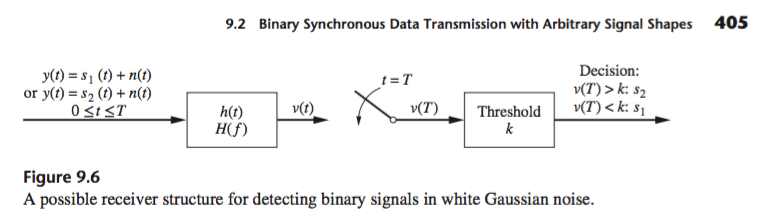
\includegraphics{Matched Filter.png}
	\end{frame}

	\begin{frame}
		\frametitle{Continuing with Probability Error}
		\begin{itemize}
			\item $\zeta_max^2 = 2/N_0*(E_1+E_2-2*\sqrt{E_1*E_2}*\rho_{12}) $
			\item And our error probability become $P_E=Q*((E_b/N_0)*(1-(\sqrt{1-\sqrt{E_1*E_2}/E *\rho_12))^(1/2)$
			\item From the derivation before we know that $E_b=1/2*(E_1+E_2)$ is the average received-signal energy, since $s_1(t)$ and $s_2(t)$ are transmitted with equal a priori probability.
			\item So we know that from our derivations, we can finally write as; $P_E$=$Q$*($\sqrt{(1-R_12)*(E_b/N_0)}$)
			\item We know that $z$=$E_b$/$N_0$ is the average energy per bit divided by noise power spectral density.
			\item Also the parameter %$R_12$= $((2*\sqrt{E_1*E_2})$/($E_1$+$E_2$))* $\rho_12
			\item Minimum value for %$R_12$= $-1$ which attained for $E_1$=$E_2$
		\end{itemize}
	\end{frame}

	\begin{frame}
		\frametitle{Correlator Implementation of the Matched- Filter Receiver}
		\begin{itemize}
			\item Optimum receiver involved the two filters with impulse responses equal to the time reverse of the respective signals has been processed.
			\item An alternative receiver structure can be obtained by nothing that the matched filter can be replaced by a multiplier-integrator cascade. Operations will be referred to as correlation detection.
			\item If we want to mathematically show the output of the matched filter;
			%$v(t)$=$h(t)$* $y(t)$= $\int_{0, T} s(T-\tau)*y(t-\tau) $d\tau$ $
			\item From there we obtain the following,% $v(t)$=$\int_{0, T} s(\alpha)*y(\alpha) $d\alpha$ $
		\end{itemize}
	\end{frame}


	\begin{frame}
		\frametitle{ Figures for the equivalence of the matched-filter and correlator receivers}
		%includegraphics{figure will come}
	\end{frame}

	\begin{frame}
		\frametitle{Optimum Threshold}
		\begin{itemize}
			\item The optimum detection filter is a matched filter, matched to the difference of the input signals has the impulse response that given by% $h_0(??)$=$g(?? ???)$=$??_2(?? ???)$?$??_1(?? ???)$
			\item From the superposition integral , we will get $\sqrt{E_1*E_2}*$\rho_12-$E_1$ for $s_01(T)$
			\item If we apply same logic on $s_02(T)$, we will get $E_2$-($\sqrt{E_1*E_2}$*$\rho_12$
			\item Substituting $s_01(T)$ and $s_02(T) , we will get optimum threshold that;
			$k_opt$=$1/2$*($E_2$-$E_1$)
			\item It is important to note that equal energy signals will result in a optimum threshold of zero.
		\end{itemize}
	\end{frame}
\end{document}
